\section[GIMP]{Verallgemeinerte implizite Mittelpunktsregel}
\begin{frame}[<+->]
\frametitle{Lösen von ODEs mittels stückweiser Linearisierung}
 \begin{block}{Verallgemeinerte implizite Mittelpunktsregel (GIMP)}
 \[
  x_n - x_a = h\int_{-\frac{1}{2}}^{\frac{1}{2}} F(\xo) + \Delta F(\xo; t(x-\xo))dt
 \]
\end{block}
Schritte:
\begin{itemize}
 \item Berechnung der kritischen Multiplikatoren
 \item Integration über stückweise lineare Funktion (exakt)
 \item Lösung des entstehenden LGS mittels Unfolded Newton System auf stückweise linearem Modell
\end{itemize}

\end{frame}

\begin{frame}[<+->]
\frametitle{Berechnung der Kritischen Multiplikatoren}
\begin{minipage}{0.5\textwidth} 
	\begin{block}{Kritische Multiplikatoren}
	 \glqq Kinks befinden sich an den Nullstellen der switching Variablen~$z$ der Abs Normal Form \grqq
	\end{block}
	\begin{block}{Berechnung}
	   Erste Zeile der Abs Normal Form\\
	   $ z = c+ Zx+L|z|$\\
	    und\\
	   $\dot z = Z\Delta x+L\Sigma \dot z, \Sigma = \diag(\sgn(z))$
	    \begin{align*}
	    \Rightarrow z_j + \tau_j \dot z_j = 0 \iff & \tau_j = -\frac{z_j}{\dot z_j}\\
						       & \dot z_j\neq 0
	    \end{align*}
	\end{block}
	\end{minipage}
	\hfill
	\begin{minipage}{0.4\textwidth}
	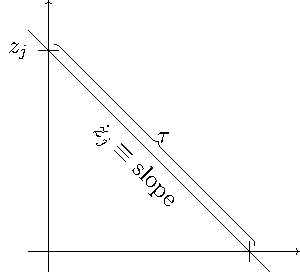
\includegraphics[width=\linewidth]{../dipl_tex/img/tikz/finding_kinks.pdf}	
	\end{minipage}
\end{frame}
\begin{frame}[<+->]
\frametitle{Berechnung der GIMP}
\begin{align}
x_n - x_a &= h \int_{-\frac{1}{2}}^{\frac{1}{2}} F(\xo) + \Delta F(\xo,t(x_n-x_a))dt\\
\iff x_n - x_a -h F(\xo)&= \underbrace{h \int_{-\frac{1}{2}}^{\frac{1}{2}} \Delta F(\xo,t(x_n-x_a))dt}_{r(x_n,x_a)}\\
x_n - x_a -h F(\xo) &= r(x_n,x_a)
\end{align}
\begin{align}
  x_n^{\text{(n)}} - x_a - h (F(\xoold) +\Delta F(\xoold,\xonew - \xoold)) &= r(x_n^{\text{(a)}},x_a)\\
 \iff 2\xonew - 2x_a - h (F(\xoold) +\Delta F(\xoold,\xonew - \xoold)) &= r(x_n^{\text{(a)}},x_a)\\
 \iff  2\xonew -  h (F(\xoold) +\Delta F(\xoold,\xonew - \xoold)) &= r(x_n^{\text{(a)}},x_a) + 2x_a
\end{align}
\[x_n = 2\xo - x_a\]
\end{frame}


